\documentclass[dvipdfmx]{standalone}
\usepackage{tikz,gnuplot-lua-tikz}
\begin{document}
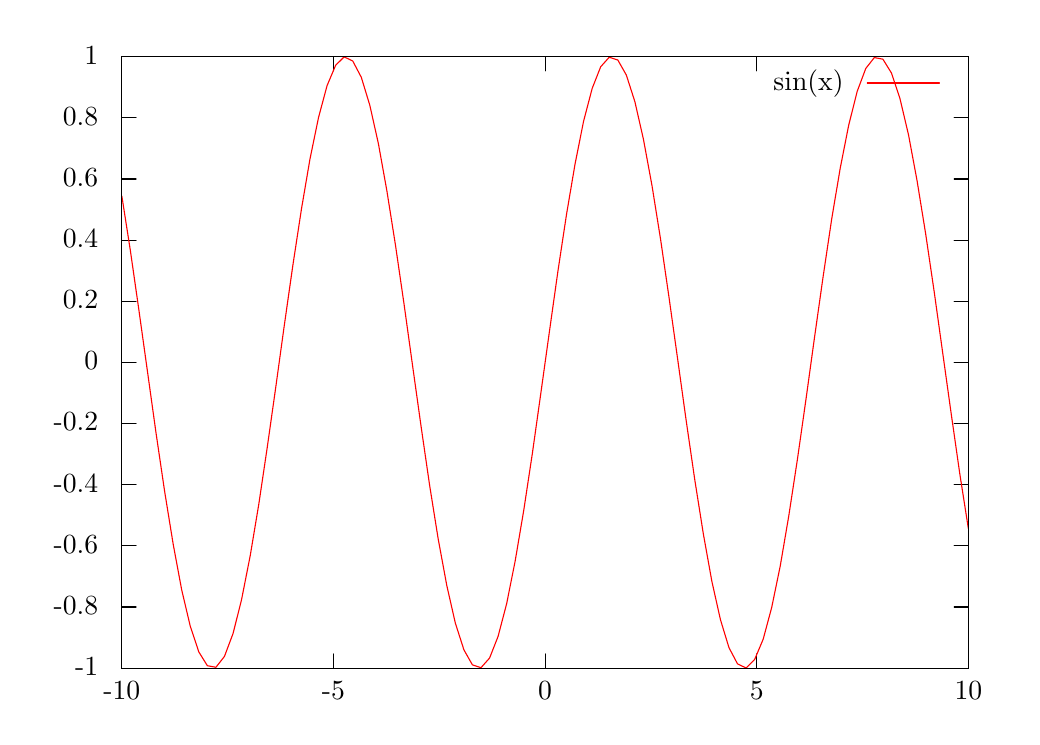
\begin{tikzpicture}[gnuplot]
%% generated with GNUPLOT 4.6p6 (Lua 5.1; terminal rev. 99, script rev. 100)
%% 2016年07月12日 18時16分15秒
\path (0.000,0.000) rectangle (12.500,8.750);
\gpcolor{color=gp lt color border}
\gpsetlinetype{gp lt border}
\gpsetlinewidth{1.00}
\draw[gp path] (1.196,0.616)--(1.376,0.616);
\draw[gp path] (11.947,0.616)--(11.767,0.616);
\node[gp node right] at (1.012,0.616) {-1};
\draw[gp path] (1.196,1.392)--(1.376,1.392);
\draw[gp path] (11.947,1.392)--(11.767,1.392);
\node[gp node right] at (1.012,1.392) {-0.8};
\draw[gp path] (1.196,2.169)--(1.376,2.169);
\draw[gp path] (11.947,2.169)--(11.767,2.169);
\node[gp node right] at (1.012,2.169) {-0.6};
\draw[gp path] (1.196,2.945)--(1.376,2.945);
\draw[gp path] (11.947,2.945)--(11.767,2.945);
\node[gp node right] at (1.012,2.945) {-0.4};
\draw[gp path] (1.196,3.722)--(1.376,3.722);
\draw[gp path] (11.947,3.722)--(11.767,3.722);
\node[gp node right] at (1.012,3.722) {-0.2};
\draw[gp path] (1.196,4.499)--(1.376,4.499);
\draw[gp path] (11.947,4.499)--(11.767,4.499);
\node[gp node right] at (1.012,4.499) { 0};
\draw[gp path] (1.196,5.275)--(1.376,5.275);
\draw[gp path] (11.947,5.275)--(11.767,5.275);
\node[gp node right] at (1.012,5.275) { 0.2};
\draw[gp path] (1.196,6.052)--(1.376,6.052);
\draw[gp path] (11.947,6.052)--(11.767,6.052);
\node[gp node right] at (1.012,6.052) { 0.4};
\draw[gp path] (1.196,6.828)--(1.376,6.828);
\draw[gp path] (11.947,6.828)--(11.767,6.828);
\node[gp node right] at (1.012,6.828) { 0.6};
\draw[gp path] (1.196,7.605)--(1.376,7.605);
\draw[gp path] (11.947,7.605)--(11.767,7.605);
\node[gp node right] at (1.012,7.605) { 0.8};
\draw[gp path] (1.196,8.381)--(1.376,8.381);
\draw[gp path] (11.947,8.381)--(11.767,8.381);
\node[gp node right] at (1.012,8.381) { 1};
\draw[gp path] (1.196,0.616)--(1.196,0.796);
\draw[gp path] (1.196,8.381)--(1.196,8.201);
\node[gp node center] at (1.196,0.308) {-10};
\draw[gp path] (3.884,0.616)--(3.884,0.796);
\draw[gp path] (3.884,8.381)--(3.884,8.201);
\node[gp node center] at (3.884,0.308) {-5};
\draw[gp path] (6.572,0.616)--(6.572,0.796);
\draw[gp path] (6.572,8.381)--(6.572,8.201);
\node[gp node center] at (6.572,0.308) { 0};
\draw[gp path] (9.259,0.616)--(9.259,0.796);
\draw[gp path] (9.259,8.381)--(9.259,8.201);
\node[gp node center] at (9.259,0.308) { 5};
\draw[gp path] (11.947,0.616)--(11.947,0.796);
\draw[gp path] (11.947,8.381)--(11.947,8.201);
\node[gp node center] at (11.947,0.308) { 10};
\draw[gp path] (1.196,8.381)--(1.196,0.616)--(11.947,0.616)--(11.947,8.381)--cycle;
\node[gp node right] at (10.479,8.047) {sin(x)};
\gpcolor{color=gp lt color 0}
\gpsetlinetype{gp lt plot 0}
\draw[gp path] (10.663,8.047)--(11.579,8.047);
\draw[gp path] (1.196,6.611)--(1.305,5.914)--(1.413,5.160)--(1.522,4.379)--(1.630,3.603)%
  --(1.739,2.863)--(1.848,2.190)--(1.956,1.610)--(2.065,1.148)--(2.173,0.823)--(2.282,0.647)%
  --(2.391,0.627)--(2.499,0.765)--(2.608,1.055)--(2.716,1.485)--(2.825,2.038)--(2.934,2.690)%
  --(3.042,3.416)--(3.151,4.186)--(3.259,4.969)--(3.368,5.733)--(3.477,6.447)--(3.585,7.081)%
  --(3.694,7.610)--(3.802,8.013)--(3.911,8.272)--(4.019,8.379)--(4.128,8.327)--(4.237,8.120)%
  --(4.345,7.765)--(4.454,7.278)--(4.562,6.677)--(4.671,5.988)--(4.780,5.238)--(4.888,4.459)%
  --(4.997,3.680)--(5.105,2.936)--(5.214,2.254)--(5.323,1.664)--(5.431,1.189)--(5.540,0.849)%
  --(5.648,0.658)--(5.757,0.622)--(5.866,0.744)--(5.974,1.019)--(6.083,1.435)--(6.191,1.976)%
  --(6.300,2.620)--(6.409,3.340)--(6.517,4.107)--(6.626,4.890)--(6.734,5.657)--(6.843,6.377)%
  --(6.952,7.021)--(7.060,7.562)--(7.169,7.978)--(7.277,8.253)--(7.386,8.375)--(7.495,8.339)%
  --(7.603,8.148)--(7.712,7.808)--(7.820,7.333)--(7.929,6.743)--(8.038,6.061)--(8.146,5.317)%
  --(8.255,4.538)--(8.363,3.759)--(8.472,3.009)--(8.581,2.320)--(8.689,1.719)--(8.798,1.232)%
  --(8.906,0.877)--(9.015,0.670)--(9.124,0.618)--(9.232,0.725)--(9.341,0.984)--(9.449,1.387)%
  --(9.558,1.916)--(9.666,2.550)--(9.775,3.264)--(9.884,4.028)--(9.992,4.811)--(10.101,5.581)%
  --(10.209,6.307)--(10.318,6.959)--(10.427,7.512)--(10.535,7.942)--(10.644,8.232)--(10.752,8.370)%
  --(10.861,8.350)--(10.970,8.174)--(11.078,7.849)--(11.187,7.387)--(11.295,6.807)--(11.404,6.134)%
  --(11.513,5.394)--(11.621,4.618)--(11.730,3.837)--(11.838,3.083)--(11.947,2.386);
\gpcolor{color=gp lt color border}
\gpsetlinetype{gp lt border}
\draw[gp path] (1.196,8.381)--(1.196,0.616)--(11.947,0.616)--(11.947,8.381)--cycle;
%% coordinates of the plot area
\gpdefrectangularnode{gp plot 1}{\pgfpoint{1.196cm}{0.616cm}}{\pgfpoint{11.947cm}{8.381cm}}
\end{tikzpicture}
\end{document}
%% gnuplot variables
